\documentclass[10pt,a4paper]{article}
\usepackage[utf8]{inputenc}
\usepackage[T1]{fontenc}
\usepackage{amsmath}
\usepackage{amsfonts}
\usepackage{amssymb}
\usepackage{graphicx}
\begin{document}
	\section{Description}
	There is a man. He can cook, eat, and play. Cooking makes food cooked. he can eat food if it is cooked. After eating he feels not hungry, and food is not cooked again. He can play. Playing makes him hungry. He just can play if he is not hungry. He just cooks when there is no food is cooked. Initially, the is hungry, and no food is cooked. In terms of energy, eating costs 5, cooking costs 15, playing costs 20.\\
	\\
	\section{Representation in language}
	Fluents: cooked, hungry.\\
	Actions: cook, eat, play.\\
	\\
	eat costs 5\\
	cooking cost 15\\
	play cost 20\\
	initially $\neg$cooked $\land$ hungry\\
	cook causes cook if $\neg$cooked\\
	eat causes ($\neg$cooked $\land$ $\neg$hungry) if cooked\\
	play causes hungry if $\neg$hungry\\
	\\
	\section{Calculation}
	$\sum$ = \{$\sigma$0 ,$\sigma$1, $\sigma$2, $\sigma$3\}\\
	\\
	$\sigma$0 = \{$\neg$cooked, hungry\}\\
	$\sigma$1 = \{cooked, hungry\}\\
	$\sigma$2 = \{$\neg$cooked, $\neg$hungry\}\\
	$\sigma$3 = \{cooked, $\neg$hungry\}\\
	\\
	$\psi$(eat, $\sigma$0) = $\sigma$0\\
	$\psi$(cook, $\sigma$0) = $\sigma$1\\
	$\psi$(play, $\sigma$0) = $\sigma$0\\
	\\
	$\psi$(eat, $\sigma$1) = $\sigma$2\\
	$\psi$(cook, $\sigma$1) = $\sigma$1\\
	$\psi$(play, $\sigma$1) = $\sigma$1\\
	\\
	$\psi$(eat, $\sigma$2) = $\sigma$2\\
	$\psi$(cook, $\sigma$2) = $\sigma$3\\
	$\psi$(play, $\sigma$2) = $\sigma$1\\
	\\
	$\psi$(eat, $\sigma$3) = $\sigma$2\\
	$\psi$(cook, $\sigma$3) = $\sigma$3\\
	$\psi$(play, $\sigma$3) = $\sigma$1\\
	\\
	\section{Graph}
	
	\begin{figure}[h]
		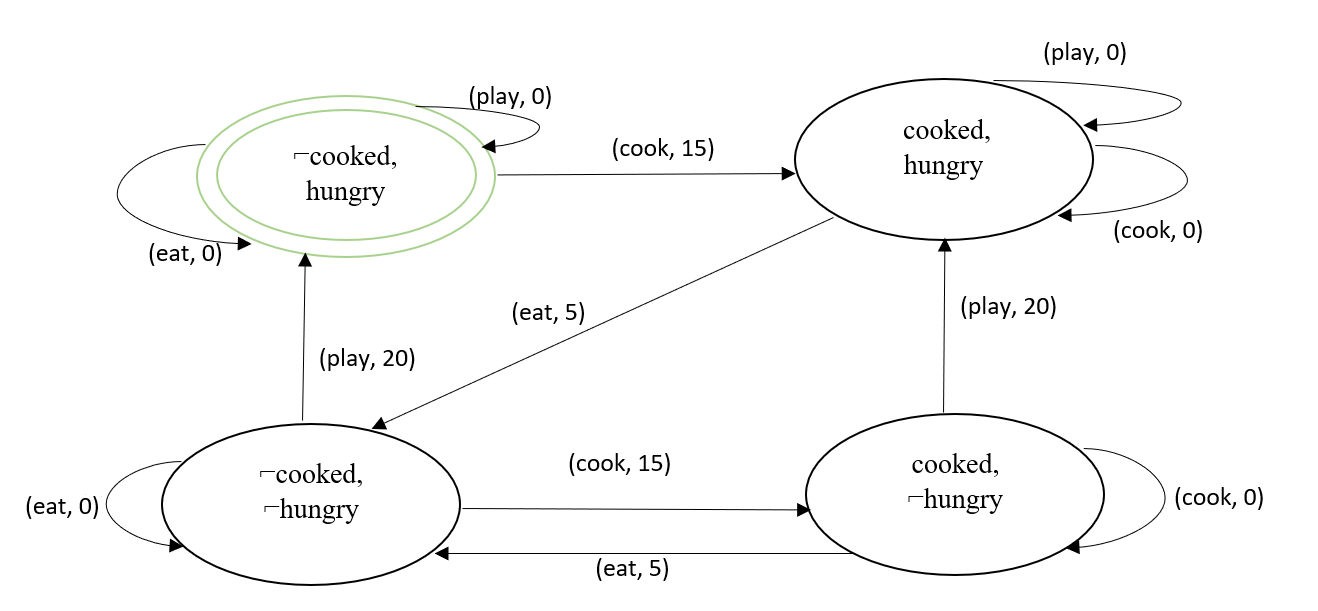
\includegraphics[width=1\linewidth, height=0.3\textheight]{figure01}
	\end{figure}
	
\end{document}